\chapter{Performance evaluation}
\label{ch:perf}

\section{Methodology}
All timings are wall-clock milliseconds on one machine, taking the \emph{best of five} runs of each program (the minimum is the least noisy estimator for short deterministic programs). CPython 3 is the reference. Each benchmark is checked for \emph{identical output} across the compared builds before timing, so a faster number can never come from computing something different. The script is \code{scripts/bench.sh}; the raw output of the report's run is in Appendix~\ref{app:bench}.

\section{Native code versus CPython}
\begin{table}[H]\centering\small\begin{tabular}{@{}lrrrrr@{}}\toprule
\textbf{Benchmark} & \textbf{CPython (ms)} & \textbf{Native, no regalloc (ms)} & \textbf{Native, regalloc (ms)} & \textbf{vs.\ CPython} & \textbf{regalloc gain}\\ \midrule
\texttt{fib35} & 654 & 74 & 54 & 12.1$\times$ & 1.37$\times$\\
\texttt{primes} & 388 & 32 & 33 & 11.7$\times$ & .96$\times$\\
\bottomrule
\end{tabular}
\caption{Native x86-64 code (without and with register allocation) versus CPython. \texttt{fib35} is the doubly-recursive Fibonacci of 35; \texttt{primes} counts primes below 300{,}000 by trial division.}\end{table}

\begin{figure}[H]\centering
\begin{tikzpicture}
\begin{axis}[ybar,width=0.9\textwidth,height=6.2cm,bar width=16pt,symbolic x coords={fib35,primes},xtick=data,ymode=log,log origin=infty,ymin=10,ymax=1500,ylabel={time (ms, log scale)},legend style={at={(0.5,-0.18)},anchor=north,legend columns=3,font=\sffamily\small},point meta=rawy,nodes near coords,every node near coord/.append style={font=\sffamily\scriptsize,/pgf/number format/.cd,fixed,precision=0},axis x line*=bottom,axis y line*=left,font=\sffamily\small,enlarge x limits=0.35]
\addplot[fill=crimson!70,draw=none] coordinates {(fib35,\BenchFibPy) (primes,\BenchPrimesPy)};
\addplot[fill=amber!80,draw=none] coordinates {(fib35,\BenchFibNoreg) (primes,\BenchPrimesNoreg)};
\addplot[fill=teal!80,draw=none] coordinates {(fib35,\BenchFibReg) (primes,\BenchPrimesReg)};
\legend{CPython,Native (no regalloc),Native (linear-scan)}
\end{axis}
\end{tikzpicture}
\caption{Run time (lower is better; logarithmic scale). Native code is about \BenchFibVspy$\times$ (fib) and \BenchPrimesVspy$\times$ (primes) faster than CPython.}
\end{figure}

\textbf{Reading the numbers.} A tree- or bytecode-interpreting language such as CPython pays dispatch overhead on every operation; native code pays none, so the large gap is expected and not a claim that NOVA is a better language. The comparison does show that the native back end produces genuinely fast code.

\section{What the register allocator buys --- and what it does not}
For \texttt{fib35}, linear-scan allocation reduces the time from \BenchFibNoreg{} ms to \BenchFibReg{} ms (\BenchFibVsnoreg$\times$). For \texttt{primes} the gain is \BenchPrimesVsnoreg$\times$ --- effectively none.

\begin{keybox}
The sieve spends almost all its time in the integer \emph{divide} instruction (\code{idiv}, the \code{\%} operator), whose latency (tens of cycles) dwarfs a few memory accesses; making the surrounding moves cheaper cannot help. \texttt{fib35}, by contrast, is a tight mix of compares, additions and calls where keeping the argument in a register removes a store-to-load dependency on every call. Reporting the null result is the honest outcome of measuring instead of assuming.
\end{keybox}

\section{Inlining}
The benchmark \texttt{benchmarks/inline.nova} runs a loop whose body calls three small helper functions (a square, a mix function and a clamp). With inlining disabled the native program takes \BenchInlineOff{} ms; with inlining enabled it takes \BenchInlineOn{} ms: a \BenchInlineGain$\times$ speed-up with identical output (\code{1000000007}).

\begin{figure}[H]\centering
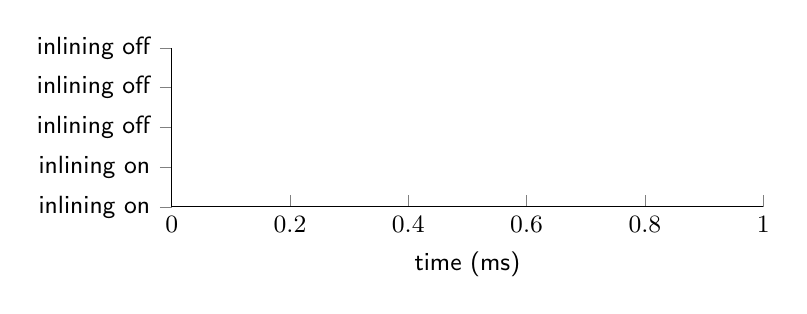
\begin{tikzpicture}
\begin{axis}[xbar,width=0.75\textwidth,height=3.6cm,bar width=14pt,xmin=0,xmax=130,symbolic y coords={inlining on,inlining off},ytick=data,nodes near coords,axis x line*=bottom,axis y line*=left,xlabel={time (ms)},enlarge y limits=0.5,font=\sffamily\small]
\addplot[fill=nova!75,draw=none] coordinates {(\BenchInlineOff,inlining off) (\BenchInlineOn,inlining on)};
\end{axis}
\end{tikzpicture}
\caption{Effect of inlining on a call-heavy loop (native code).}
\end{figure}

\section{Effect of the optimizer on the random-program corpus}
Over \FuzzN{} generated programs the optimizer reduced the total IR from \FuzzIRBefore{} to \FuzzIRAfter{} instructions (\FuzzIRCut{}\%) and the work executed by the VM from \FuzzStepsBefore{} to \FuzzStepsAfter{} steps (\FuzzStepCut{}\%), with no behavioural difference. The generated programs contain a lot of constant arithmetic by construction, so these percentages illustrate the machinery rather than predicting gains on real code.

\pgfmathsetmacro{\IRRemain}{100-\FuzzIRCut}\pgfmathsetmacro{\StepRemain}{100-\FuzzStepCut}
\begin{figure}[H]\centering
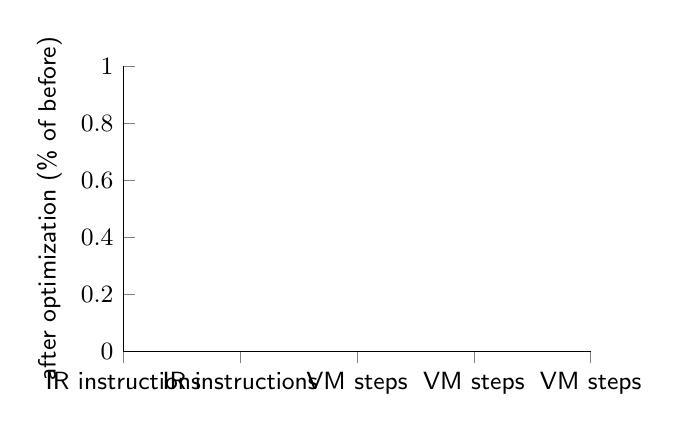
\begin{tikzpicture}
\begin{axis}[ybar,width=0.62\textwidth,height=5.2cm,bar width=26pt,symbolic x coords={IR instructions,VM steps},xtick=data,ymin=0,ymax=105,ylabel={after optimization (\% of before)},nodes near coords,every node near coord/.append style={font=\sffamily\small},axis x line*=bottom,axis y line*=left,font=\sffamily\small,enlarge x limits=0.5]
\addplot[fill=teal!75,draw=none] coordinates {(IR instructions,\IRRemain) (VM steps,\StepRemain)};
\end{axis}
\end{tikzpicture}
\caption{Remaining work after optimization on \FuzzN{} random programs.}
\end{figure}

\section{Static effect of register allocation}
For the shipped Fibonacci example the allocator reduces instructions that touch the stack from \AsmMemOff{} to \AsmMemOn{} (\AsmMemCut{}\%), while total instruction count rises from \AsmInstrOff{} to \AsmInstrOn{} because of the callee-saved register saves and restores. Fewer, but more expensive, instructions are replaced by more, but cheaper, ones.

\section{Compilation speed}
Compiling and running the \NumExamples{} shipped programs takes \CompileMsAvg{} ms on average (\CompileMsMax{} ms for the slowest), summing the time of all seven compiler stages. About \LRBuildMs{} ms of every run is spent \emph{building the LR(1) tables} from the grammar at start-up --- so for small programs the parser generator, not the compiler, dominates.

\begin{warnbox}
Caching or pre-generating the LR(1) tables would remove roughly \LRBuildMs{} ms from every compiler start. It was not done because building the tables at start-up keeps the grammar text as the single source of truth and the cost is invisible in the studio, but it is the first optimization to make if \code{novac} were used in a build system.
\end{warnbox}
